\clearpage
\section{Visual walkthrough: follow the loops through the matrix}
The drawings use a four-bit teaching matrix so every cell remains visible.
The real function uses the same indexing and operations with 32 bits. The small
matrix below is invertible, but it is not the SM4 linear transformation.

\definecolor{walkblue}{HTML}{DBEAFE}
\definecolor{walkteal}{HTML}{CCFBF1}
\definecolor{walkorange}{HTML}{FED7AA}
\newcommand{\walkmatrix}[2]{%
\begin{tikzpicture}[x=7mm,y=7mm,every node/.style={font=\small}]
\foreach \r/\a/\b/\c/\d in {0/1/1/0/0,1/0/1/1/0,2/1/0/0/0,3/0/0/0/1}{%
  \foreach \j/\v in {0/\a,1/\b,2/\c,3/\d}{%
    \def\shade{white}%
    \ifnum\j=#2\relax\def\shade{walkblue}\fi%
    \ifnum\r=#1\relax\def\shade{walkteal}\fi%
    \ifnum\r=#1\relax\ifnum\j=#2\relax\def\shade{walkorange}\fi\fi%
    \node[draw,fill=\shade,minimum width=7mm,minimum height=7mm] at (\j,-\r) {\v};%
  }%
  \node[left] at (-0.6,-\r) {$r=\r$};%
}%
\foreach \j in {0,1,2,3}{\node at (\j,0.9) {$\j$};}%
\node at (1.5,1.85) {\hx{column\_index}};
\draw[-{Stealth},thick,orange!80!black] (#2,1.5)--(#2,1.1);
\end{tikzpicture}}

\subsection{First understand the two directions}
\begin{center}
\walkmatrix{1}{2}
\end{center}
\begin{center}\begin{tabular}{ll}\toprule
Teal row & The outer loop fixes \hx{row\_index = 1}.\\
Blue column & The inner loop currently uses \hx{column\_index = 2}.\\
Orange cell & We read $M[1,2]=1$.\\\bottomrule
\end{tabular}\end{center}

\begin{Verbatim}
for row_index in range(4):        # move DOWN to the next row
    matrix_row = 0
    for column_index in range(4): # move RIGHT across this row
        output_bit = (columns[column_index] >> row_index) & 1
        matrix_row |= output_bit << column_index
\end{Verbatim}
\noindent The actual file uses \hx{range(32)}. While the inner loop runs,
\hx{row\_index} does not change. The visited cells are
\[
(0,0)\to(0,1)\to(0,2)\to(0,3),\quad
(1,0)\to(1,1)\to(1,2)\to(1,3),\quad\ldots
\]
The arrays already contain columns; these loops collect their bits into rows.
They do not move or modify the original matrix entries.

\subsection{Matrix order and printed binary order are different}
Matrix columns are drawn left-to-right as $c=0,1,2,3$. A printed binary integer
is written with its highest bit first: $b_3b_2b_1b_0$.
The highlighted matrix row is $[0,1,1,0]$. Its packed value is
$0\cdot2^0+1\cdot2^1+1\cdot2^2+0\cdot2^3=6$, printed as \hx{0110}.
For row 0, $[1,1,0,0]$ is printed as \hx{0011}, not \hx{1100}.
\note{A shift operates on the stored integer. It does not slide a matrix cell
visually to the right. The bit index tells us which coefficient to extract.}

\clearpage
\subsection{One column is an integer: why shift and AND?}
Column 0 of the teaching matrix contains these entries from top to bottom:
\begin{center}
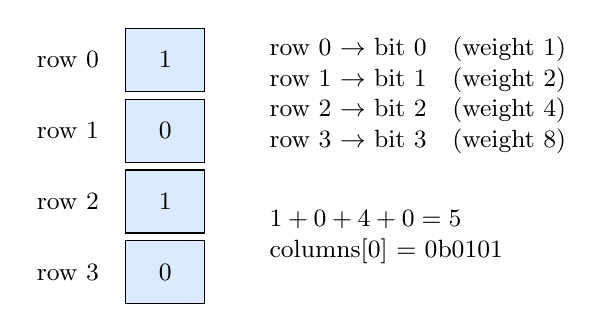
\begin{tikzpicture}[x=12mm,y=9mm,every node/.style={font=\small}]
\foreach \r/\v in {0/1,1/0,2/1,3/0}{
\node[draw,fill=walkblue,minimum width=10mm,minimum height=8mm] at (0,-\r) {\v};
\node[left] at (-0.6,-\r) {row \r};
}
\node[align=left,anchor=west] at (1,-0.5) {row 0 $\to$ bit 0\quad(weight 1)\\row 1 $\to$ bit 1\quad(weight 2)\\row 2 $\to$ bit 2\quad(weight 4)\\row 3 $\to$ bit 3\quad(weight 8)};
\node[align=left,anchor=west] at (1,-2.5) {$1+0+4+0=5$\\\hx{columns[0] = 0b0101}};
\end{tikzpicture}
\end{center}
To read row 2 from this column, shift its bit into position 0, then keep only
that position. Every number below is a four-bit binary word:
\begin{center}
\begin{tikzpicture}[x=10mm,y=9mm,every node/.style={font=\small}]
\foreach \j/\bit in {0/3,1/2,2/1,3/0}{\node at (\j,0.9) {bit \bit};}
\foreach \j/\v in {0/0,1/1,2/0,3/1}{\node[draw,minimum size=8mm] at (\j,0) {\v};}
\node[right] at (4,0) {\hx{0101}: original column};
\foreach \j/\v in {0/0,1/0,2/0,3/1}{\node[draw,fill=walkteal,minimum size=8mm] at (\j,-1.5) {\v};}
\node[right] at (4,-1.5) {\hx{0001}: after \hx{>> 2}};
\draw[-{Stealth},orange!90!black,thick] (1,-0.45)--(3,-1.05);
\node[below,align=center] at (1.5,-2.3) {The selected bit reaches position 0.\\AND with \hx{0001} discards every other bit.};
\end{tikzpicture}
\end{center}
\[
(\texttt{0101}\gg2)\mathbin{\&}\texttt{0001}
=\texttt{0001}\mathbin{\&}\texttt{0001}=1.
\]
For row 1, instead:
\[
(\texttt{0101}\gg1)\mathbin{\&}\texttt{0001}
=\texttt{0010}\mathbin{\&}\texttt{0001}=0.
\]
The other surviving 1 in \hx{0010} does not matter: AND with 1 tests only the
least significant bit. This is why shifting alone is insufficient.

The four stored columns of this matrix are:
\begin{center}\begin{tabular}{ccccc}\toprule
Index & 0 & 1 & 2 & 3\\\midrule
Top-to-bottom entries & $[1,0,1,0]$ & $[1,1,0,0]$ & $[0,1,0,0]$ & $[0,0,0,1]$\\
Stored binary & \hx{0101} & \hx{0011} & \hx{0010} & \hx{1000}\\\bottomrule
\end{tabular}\end{center}

\clearpage
\subsection{Four iterations: build row 1 from left to right}
Keep \hx{row\_index = 1}. Start with \hx{matrix\_row = 0000}.
Each orange cell is the next bit read; all binary words below have four bits.

\noindent\begin{minipage}[t]{.48\linewidth}\centering
\textbf{Iteration 1: column 0}\par\medskip
\walkmatrix{1}{0}\par
Read $(\hx{0101}\gg1)\mathbin{\&}1=0$.\par
Position it: $0\ll0=\hx{0000}$.\par
Accumulate: $\hx{0000}\,|\,\hx{0000}=\hx{0000}$.
\end{minipage}\hfill
\begin{minipage}[t]{.48\linewidth}\centering
\textbf{Iteration 2: column 1}\par\medskip
\walkmatrix{1}{1}\par
Read $(\hx{0011}\gg1)\mathbin{\&}1=1$.\par
Position it: $1\ll1=\hx{0010}$.\par
Accumulate: $\hx{0000}\,|\,\hx{0010}=\hx{0010}$.
\end{minipage}

\bigskip\bigskip
\noindent\begin{minipage}[t]{.48\linewidth}\centering
\textbf{Iteration 3: column 2}\par\medskip
\walkmatrix{1}{2}\par
Read $(\hx{0010}\gg1)\mathbin{\&}1=1$.\par
Position it: $1\ll2=\hx{0100}$.\par
Accumulate: $\hx{0010}\,|\,\hx{0100}=\hx{0110}$.
\end{minipage}\hfill
\begin{minipage}[t]{.48\linewidth}\centering
\textbf{Iteration 4: column 3}\par\medskip
\walkmatrix{1}{3}\par
Read $(\hx{1000}\gg1)\mathbin{\&}1=0$.\par
Position it: $0\ll3=\hx{0000}$.\par
Accumulate: $\hx{0110}\,|\,\hx{0000}=\hx{0110}$.
\end{minipage}

\bigskip
The inner loop has reconstructed row 1: matrix entries $[0,1,1,0]$, stored as
integer 6, binary \hx{0110}. OR accumulates set bits; OR with zero preserves
the bits already written. Only after the inner loop finishes does the outer
loop move down to row 2 and reset \hx{matrix\_row = 0}.

\begin{center}
\begin{tikzpicture}[every node/.style={font=\small},node distance=4mm]
\node[draw,fill=walkblue,align=center] (a) {choose column\\\hx{columns[c]}};
\node[draw,fill=walkorange,right=of a,align=center] (b) {extract row bit\\\hx{>> r}, then \hx{\& 1}};
\node[draw,fill=walkteal,right=of b,align=center] (c) {place column bit\\\hx{<< c}, then OR};
\draw[-{Stealth}] (a)--(b);\draw[-{Stealth}] (b)--(c);
\end{tikzpicture}
\end{center}

\clearpage
\subsection{Where does the identity go in the packed row?}
With four bits per half, the code's \hx{32 + row\_index} becomes
\hx{4 + row\_index}. For row 1, the identity's 1 belongs at position 5:
\[
\hx{identity\_bit}=1\ll(4+1)=\texttt{00100000}.
\]
\begin{center}
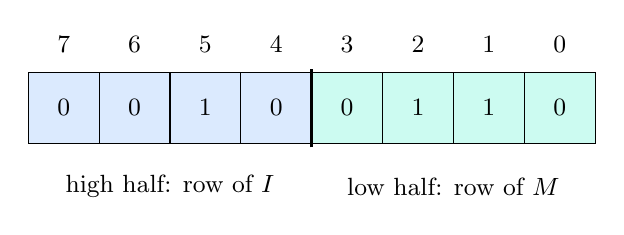
\begin{tikzpicture}[x=9mm,y=10mm,every node/.style={font=\small}]
\foreach \j/\bit/\v in {0/7/0,1/6/0,2/5/1,3/4/0,4/3/0,5/2/1,6/1/1,7/0/0}{
\def\shade{walkblue}\ifnum\j>3\def\shade{walkteal}\fi
\node[draw,fill=\shade,minimum size=9mm] at (\j,0) {\v};
\node at (\j,.8) {\bit};
}
\draw[very thick] (3.5,-.5)--(3.5,.5);
\node at (1.5,-1) {high half: row of $I$};
\node at (5.5,-1) {low half: row of $M$};
\end{tikzpicture}
\end{center}
\[
\underbrace{\texttt{00000110}}_{\text{matrix row}}
\ \big|\ \underbrace{\texttt{00100000}}_{\text{identity bit}}
=\underbrace{\texttt{00100110}}_{\text{packed augmented row}}.
\]
Mathematics writes $[M\mid I]$, but the integer above is printed high-to-low
as $[I\mid M]$. This is a storage convention, not a different algorithm.
For 32-bit SM4 halves the same structure uses 64 bit positions.

\subsection{The elimination loop walks differently}
The \hx{column} loop now chooses a pivot column, rather than collecting a row.
\hx{candidate\_row} searches down that column from the diagonal.
After a pivot is found, \hx{row} scans all other rows to eliminate their 1s.
\begin{center}
\begin{tikzpicture}[x=11mm,y=9mm,every node/.style={font=\small}]
\foreach \r/\a/\b/\c/\d in {0/1/1/0/0,1/0/1/1/0,2/1/0/0/0,3/0/0/0/1}{
\foreach \j/\v in {0/\a,1/\b,2/\c,3/\d}{
\def\shade{white}\ifnum\j=0\def\shade{walkblue}\fi
\ifnum\r=0\def\shade{walkteal}\fi
\node[draw,fill=\shade,minimum width=11mm,minimum height=9mm] at (\j,-\r) {\v};}
\node[left] at (-.6,-\r) {$R_{\r}$};}
\node[right,align=left] at (4,0) {pivot row: keep it};
\node[right,align=left] at (4,-1) {column 0 is 0: skip};
\node[right,align=left] at (4,-2) {column 0 is 1: XOR pivot};
\node[right,align=left] at (4,-3) {column 0 is 0: skip};
\draw[-{Stealth},thick,orange!90!black] (-1.1,-.2)--(-1.1,-2);
\end{tikzpicture}
\end{center}
Here $R_2\gets R_2\xor R_0$. Its matrix entries change from
$[1,0,0,0]$ to $[0,1,0,0]$. Stored as integers, the XOR is
$\hx{0001}\xor\hx{0011}=\hx{0010}$. The identity half must change too:
\[
\texttt{01000001}\xor\texttt{00010011}=\texttt{01010010}.
\]
After all pivot columns, the low half is identity and the high half is inverse.
The final \hx{>> 4} (\hx{>> 32} in SM4) keeps the high half and discards the low.

\clearpage
\subsection{Finally, walk through the inverse matrix with the input vector}
For this teaching matrix, Gaussian elimination gives
\[
M^{-1}=\begin{bmatrix}
0&0&1&0\\1&0&1&0\\1&1&1&0\\0&0&0&1
\end{bmatrix}.
\]
Let $y=[1,1,1,0]^T$, stored as \hx{0111}. Each loop iteration selects one
inverse row and calculates a single output bit. This is a row--vector dot
product over GF(2), not another matrix inversion.
\begin{center}
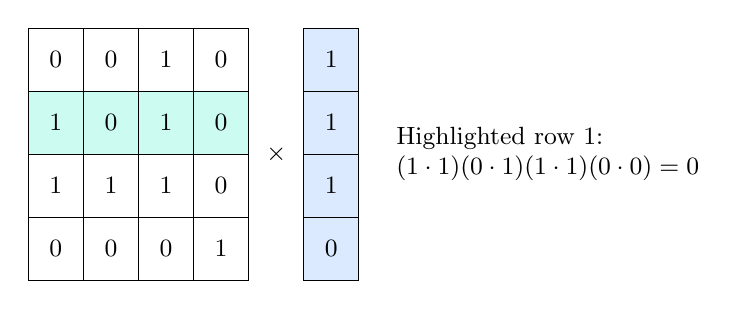
\begin{tikzpicture}[x=7mm,y=8mm,every node/.style={font=\small}]
\foreach \r/\a/\b/\c/\d in {0/0/0/1/0,1/1/0/1/0,2/1/1/1/0,3/0/0/0/1}{
\foreach \j/\v in {0/\a,1/\b,2/\c,3/\d}{
\def\shade{white}\ifnum\r=1\def\shade{walkteal}\fi
\node[draw,fill=\shade,minimum width=7mm,minimum height=8mm] at (\j,-\r) {\v};}}
\foreach \r/\v in {0/1,1/1,2/1,3/0}{\node[draw,fill=walkblue,minimum width=7mm,minimum height=8mm] at (5,-\r) {\v};}
\node at (4,-1.5) {$\times$};
\node[right,align=left] at (6,-1.5) {Highlighted row 1:\\$(1\cdot1)\xor(0\cdot1)\xor(1\cdot1)\xor(0\cdot0)=0$};
\end{tikzpicture}
\end{center}

\begin{center}\begin{tabular}{cccccc}\toprule
Index & Packed row & Input & AND & Ones / parity & Running result\\\midrule
0 & \hx{0100} & \hx{0111} & \hx{0100} & 1 / 1 & \hx{0001}\\
1 & \hx{0101} & \hx{0111} & \hx{0101} & 2 / 0 & \hx{0001}\\
2 & \hx{0111} & \hx{0111} & \hx{0111} & 3 / 1 & \hx{0101}\\
3 & \hx{1000} & \hx{0111} & \hx{0000} & 0 / 0 & \hx{0101}\\\bottomrule
\end{tabular}\end{center}
The output is $x=[1,0,1,0]^T$, stored as \hx{0101}. Forward multiplication
$Mx$ restores $y=[1,1,1,0]^T$, so the inverse result is checked.

\begin{center}\begin{tabular}{p{.36\linewidth}p{.53\linewidth}}\toprule
Loop / operation & Picture to remember\\\midrule
\hx{bit\_index} & Feed one unit vector; obtain one column.\\
\hx{row\_index}, \hx{column\_index} & Fix a row; scan its cells left-to-right.\\
\hx{>> row\_index}, then \hx{\& 1} & Bring one column bit to position 0; isolate it.\\
\hx{<< column\_index}, then OR & Place that bit in the packed output row.\\
\hx{column}, \hx{candidate\_row} & Choose a pivot column; search downward.\\
\hx{rows[row] \^{}= rows[column]} & XOR the entire augmented row, both halves.\\
\hx{augmented\_row >> 32} & Keep the inverse half after elimination.\\
\hx{index, row} in \hx{inverse\_linear} & Select one inverse row; calculate one output bit.\\\bottomrule
\end{tabular}\end{center}
\note{In the real SM4 example, the same procedure gives
$L^{-1}(\hx{734E3D3D})=\hx{4F000000}$. The four-bit drawings illustrate storage
and traversal; they do not replace the real 32-bit map.}
\clearpage
